\documentclass[tikz,border=10pt]{standalone}
\usepackage{pgfplots}
\pgfplotsset{compat=1.18}
\usepackage{amsmath}
\usepackage{amssymb}
\definecolor{mantis}{RGB}{0, 105, 62}
\begin{document}
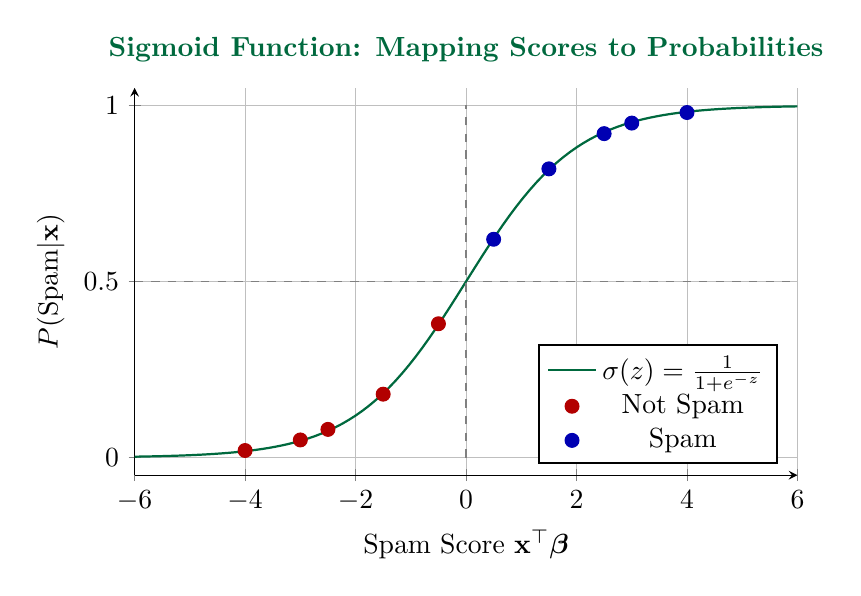
\begin{tikzpicture}
\begin{axis}[
    width=10cm,
    height=6.5cm,
    xlabel={Spam Score $\mathbf{x}^\top\boldsymbol{\beta}$},
    ylabel={$P(\text{Spam} | \mathbf{x})$},
    xmin=-6, xmax=6,
    ymin=-0.05, ymax=1.05,
    grid=both,
    grid style={line width=.1pt, draw=gray!30},
    major grid style={line width=.2pt,draw=gray!50},
    axis lines=left,
    legend pos=south east,
    title={\textbf{Sigmoid Function: Mapping Scores to Probabilities}},
    title style={font=\bfseries\color{mantis}},
]
\addplot[domain=-6:6, samples=100, color=mantis, thick] {1/(1+exp(-x))};
\addplot[dashed, gray] coordinates {(0, 0) (0, 1)};
\addplot[dashed, gray] coordinates {(-6, 0.5) (6, 0.5)};
\addplot[only marks, mark=*, mark size=2.5pt, color=red!70!black] coordinates {
    (-4, 0.02) (-3, 0.05) (-2.5, 0.08) (-1.5, 0.18) (-0.5, 0.38)
};
\addplot[only marks, mark=*, mark size=2.5pt, color=blue!70!black] coordinates {
    (0.5, 0.62) (1.5, 0.82) (2.5, 0.92) (3, 0.95) (4, 0.98)
};
\legend{$\sigma(z) = \frac{1}{1+e^{-z}}$, , , Not Spam, Spam}
\end{axis}
\end{tikzpicture}
\end{document}
